\documentclass[acmtog]{acmart}
\usepackage{algorithm}
\usepackage{algorithmicx}
\usepackage{algpseudocode}
\usepackage{graphicx}
\usepackage{subfigure}
\usepackage{natbib}
\usepackage{listings}
\usepackage{bm}
\definecolor{blve}{rgb}{0.3372549 , 0.61176471, 0.83921569}
\definecolor{gr33n}{rgb}{0.29019608, 0.7372549, 0.64705882}
\makeatletter
\lst@InstallKeywords k{class}{classstyle}\slshape{classstyle}{}ld
\makeatother
\lstset{language=C++,
	basicstyle=\ttfamily,
	keywordstyle=\color{blve}\ttfamily,
	stringstyle=\color{red}\ttfamily,
	commentstyle=\color{magenta}\ttfamily,
	morecomment=[l][\color{magenta}]{\#},
	classstyle = \bfseries\color{gr33n}, 
	tabsize=2
}
\lstset{basicstyle=\ttfamily}

% Title portion
\title{Final Project:\\ {Your Topic}}

\author{
Group Number:\quad NAN \\
Member 1:\quad Student 1\\
Member 2:\quad Student 2\\
Member 3:\quad Student 3
}

% Document starts
\begin{document}
\maketitle

\vspace*{2 ex}

\section{Section 1}

\section{Section 2}
\subsection{Residual Ratio Tracking}
Ratio tracking and residual tracking,a way that is able to handle media with wavelength dependent extinction, can be combined to compute unbiased,low-variance transmittance estimates in general heterogeneous media.To be more specfic,ratio tracking is to leverage the information discovered during the tracking more efficiently instead of deducing “just” a binary answer,finally provides a piecewise constant approximation to the transmittance function.Residual tracking,in the other hand,is complementary to delta tracking and ratio tracking and combines numerical estimation with an analytic approximation, yielding a piecewise exponential solution.
\subsubsection{Ratio Tracking}
\paragraph {\textbf{Definition}}
Ratio tracking is defined by following rules: 1.Replacing the Russian roulette by a weight that is equal to the probability of colliding with a fictitious particle. 2.Continuing the random walk until it reaches the end-point of the ray instead of probabilistically terminating the random walk at one of tentative collision points. 3.keeping track of the joint probability of colliding points with fictitious particles at all the preceding tentative collisions during the construction.By following the above rules, we can define the transmittance when reading d as:
\begin{equation}
	\begin{aligned}
	T(d)=\prod_{i=1}^{K}(1-\frac{\mu(x_{i})}{\bar{\mu}})
	\end{aligned}
\end{equation}
The multiplicand in the product represents the ratio of fictitious to all particles at collision point $x_i$.
\\Algorithm 1 is the pseudo-code of ratio tracking:
\begin{algorithm}[h]
	\caption{Pseudocode of the ratio tracking estimator of transmittance
		along a ray with origin $o$, direction $\omega$, and length $d$.}
	\begin{algorithmic}[1]
	\Function{RatioTrackingEstimator}{$o,\omega,d$}
		\State $t=0$
		\State $T=1$
		\State \textbf{do:}
			\State  \qquad$\zeta=rand() $
			\State  \qquad$t=t-\frac{log(1-\zeta)}{\bar{\mu}} $
			\State  \qquad\textbf{if} $t\geq d:$ \textbf{break}
			\State  \qquad$T = T *(1-\frac{\mu(o+t*\omega)}{\bar{\mu}}) $
			\State \textbf{while} true
			\State \textbf{return} T
	\EndFunction  
\end{algorithmic}
\end{algorithm}\\

\paragraph {\textbf{Unbiasedness of Ratio Tracking}}
The unbiasedness of Ratio Tracking can be demonstrated if it follows the following equation:
\begin{equation}
	\begin{aligned}
		E[T] = exp(-\int_{0}^{d}\mu(x)dx) = T(d)
	\end{aligned}
\end{equation}
Now we try to prove that conclusion.
Denoting $tau_i$ realizations of $T_i$,the expected value of T can be written as:
\begin{equation}
	\begin{aligned}
		E[T] = E[\sum_{i=0}^{\infty}T_i]=\sum_{i=0}^{\infty}E[T_i]=\sum_{i=0}^{\infty}\int_{i=0}^{\infty}\tau_i dP(\tau_i)
	\end{aligned}
\end{equation}
To list $T_0$ and $T_1$ as example,$T_0$ represents all realizations with the first tentative free flight distance $S_1$ already exceeding $d$.Since the value of $T_0$ equals to 1,the expected value reduces to the probability of $S_1$ taking on values greater than $d$:
\begin{equation}
	\begin{aligned}
	E[T_0] = P(S_1> d) = \int_{d}^{\infty}\tau_i dP(\tau_i)p_s(x)dx = exp(-\bar{\mu}d)
	\end{aligned}
\end{equation}
In the case of $T_1$, which represents events where $S_1 \leq d$ and $S_2 \geq -S_1$,then the expectancy of $T_1$ reads:
\begin{equation}
	\begin{aligned}
		E[T_1] &= \int_{0}^{d}\iota(x) P(S_2>d-x)dP(S_1\leq x)\\
			   &= \int_{0}^{d}\iota(x_1) P_s(x_1)\int_{d-x1}^{\infty}p_s(x_2)dx_2dx_1\\
			   &= \int_{0}^{d}\iota(x_1) \bar{\mu} exp(-\bar{\mu x_1})exp(-\bar \mu(d-x_1))dx_1\\
		   	   &=\bar{\mu}exp(-\bar{\mu}d)\int_{0}^{d}\iota(x)dx\\
	\end{aligned}
\end{equation}
Then we can analogously express the expected value of $T_k$, where represents realizations that satisfy $C_k \leq d$ and $C_k+1 >d-C_k$,as:
\begin{equation}
	\begin{aligned}
		E[T_k] &= \int_{0}^{d}\iota(x_1) P_s(x_1)\int_{0}^{d-x_1}\iota(x_1+x_2) P_s(x_2)...\\&...
		\int_{0}^{d-\sum_{j=1}^{k-1}x_j}\iota (\sum_{j=1}^{k}x_j)p_s(x_k)\\
		&\times\int_{d-\sum_{j=1}^{k-1}x_j}^{\infty}p_s(x_{k+1})dx_{k+1}dx_k...dx_2dx_1\\
		&=\int_{0}^{d}\iota(x_1)\int_{0}^{d-x_1}\iota(x_1+x_2)...\int_{0}^{d-\sum_{j=1}^{k-1}x_j}\iota (\sum_{j=1}^{k}x_j) \\
		&\times\int_{d-\sum_{j=1}^{k-1}x_j}^{\infty}\bar{\mu}^kexp(-\bar{\mu}(x_1+...x_k+(d-\sum_{j=1}^{k}x_j)))\\&dx_{k+1}dx_k...dx_2dx_1\\
		&=\bar{\mu}^kexp(-\bar{\mu}d)\int_{0}^{d}\iota(x_1)\int_{0}^{d-x_1}\iota(x_1+x_2)...\\
		&...\int_{0}^{d-\sum_{j=1}^{k-1}x_j}\iota (\sum_{j=1}^{k}x_j)dx_k...dx_2dx_1\\
	\end{aligned}
\end{equation}
Then we replace $z_i$ for $\sum_{j=0}^{i}x_j$ to rewrite the equation as:
\begin{equation}
	\begin{aligned}
		E[T_k]&=\bar{\mu}^kexp(-\bar{\mu}d)\int_{0}^{d}\iota(z_1)\int_{0}^{d-z_1}\iota(z_2)...\\
		&...\int_{0}^{d-z_{k-1}}\iota (z_k)dz_k...dz_2dz_1\\
	\end{aligned}
\end{equation}
The multiple integrals integrate $\prod_{j=1}^{k}\iota(z_j) $ over a k-dimensional simplex, which can be written concisely as:
\begin{equation}
	\begin{aligned}
		E[T_k]&=\bar{\mu}^kexp(-\bar{\mu}d)\frac{(\int_{0}^{d}\iota(x)dx)^k}{k!}
	\end{aligned}
\end{equation}
Finally,we express the expected value of T as following:
]\begin{equation}
	\begin{aligned}
		E[T]&=\sum_{k=0}^{\infty}E[T_k]\\
			&=\sum_{k=0}^{\infty}\bar{\mu}^kexp(-\bar{\mu}d)\frac{(\int_{0}^{d}\iota(x)dx)^k}{k!}\\
			&=exp(-\bar{\mu}d)\sum_{k=0}^{\infty}\frac{(\bar{\mu}\int_{0}^{d}\iota(x)dx)^k}{k!}\\
			&=exp(-\bar{\mu}d)exp(\bar{\mu}\int_{0}^{d}1-\frac{\mu(x)}{\bar{\mu}}dx)\\
			&=exp(-\int_{0}^{d}\bar{\mu}dx)exp(\int_{0}^{d}\bar{\mu}-\mu(x)dx)\\
			&=exp(-\int_{0}^{d}{\mu}(x)dx)
	\end{aligned}
\end{equation}
Though ratio tracking is unbiased, its weakness is also obvious:the expected number of steps required to reach the endpoint of the ray is high,which directly depends on the value of the majorant extinction coefficient.That's why we introduce residual tracking.
\subsubsection{Residual Tracking}
\paragraph {\textbf{Definition}}
Before introducing the definition of residual trakcing, we first analyize the transmittion function,where $\mu_c(x)$ is the extinction coefficient which is a simplified version of the original $\mu(x)$ that enables expressing the optical thickness up to distance $d$ in closed form $\tau_c(d)$:
]\begin{equation}
	\begin{aligned}
		T(d)&=exp(-\int_{0}^{d}\mu(x)dx)\\
			&=exp(-\int_{0}^{d}\mu_c(x)+\mu(x)-\mu_c(x)dx)\\
			&=exp(-\tau_c(d)) exp(-\int_0^d\mu(x)-\mu_c(x)dx)
	\end{aligned}
\end{equation}
The first exponential term, referred to as the control transmittance $T_c(d)$, represents a coarse approximation of $T(d)$, which is computed using the simplified extinction coefficient $\mu_c$. The second exponential then serves as a correction that accounts for the difference between the control and the actual transmittance. We denote
this exponential as the residual transmittance$ T_r$ and refer to the integrand as the residual extinction coefficient $\mu_r(x) = \mu(x)-\mu_c(x)$.
There is also one thing worth noticing---- in certain situations—depending on the value of $\mu_c(x)$—the residual extinction may be negative.
\\Algorithm 2 is the pseudo-code of residual ratio tracking:
\begin{algorithm}[h]
	\caption{Pseudocode of the residual ratio tracking estimator for sampling transmittance along a ray with origin $o$, direction $\omega$, and length $d$.}
	\begin{algorithmic}[1]
		\Function{ResidualRatioTrackingEstimator}{$o,\omega,d$}
		\State $t=0$
		\State $T_c=exp(-\mu_c*d)$
		\State $T_r=1$
		\State \textbf{do:}
		\State  \qquad$\zeta=rand() $
		\State  \qquad$t=t-\frac{log(1-\zeta)}{\bar{\mu_r}} $
		\State  \qquad\textbf{if} $t\geq d:$ \textbf{break}
		\State  \qquad$T_r = T_r *(1-\frac{\mu(o+t*\omega)-\mu_c}{\bar{\mu_r}}) $
		\State \textbf{while} true
		\State \textbf{return} $T_c*T_r$
		\EndFunction  
	\end{algorithmic}
\end{algorithm}\\
\paragraph{\textbf{Expression}}
According to the equation metioned before, we can obtain the residual ratio tracking estimator as below:
]\begin{equation}
	\begin{aligned}
		\left<T_r(d)\right>_{RR} = \prod_{i=1}^{K}(1-\frac{\mu_r(x_i)}{\bar{\mu_r}}) = \prod_{i=1}^{K}(1-\frac{\mu(x_i)-\mu_c}{\bar{\mu_r}})
	\end{aligned}
\end{equation}
As our goal is to minimize the tracking cost by prolonging the tentative free-flight distances, it yields to finding the smallest $\bar{\mu_r}$ that still avoids negative multiplicands,which would prevent convergence of the above estimator.To ensure that $\mu_r(x)/\bar{\mu_r} \leq 1$, we set $\bar{\mu_r} = max(|\mu_r(x)|;0\leq x \leq d)$,i.e. the maximum absolute difference between $\mu(x)$ and $\mu_c$ along the ray.


For different values of $\mu_c$, the visiulization of them is totally different,shown in the following figure, where the bright regions correspond to cases when the residual transmittance takes on values higher than 1 to correct for the overly low control transmittance.
\begin{figure}[htbp]
	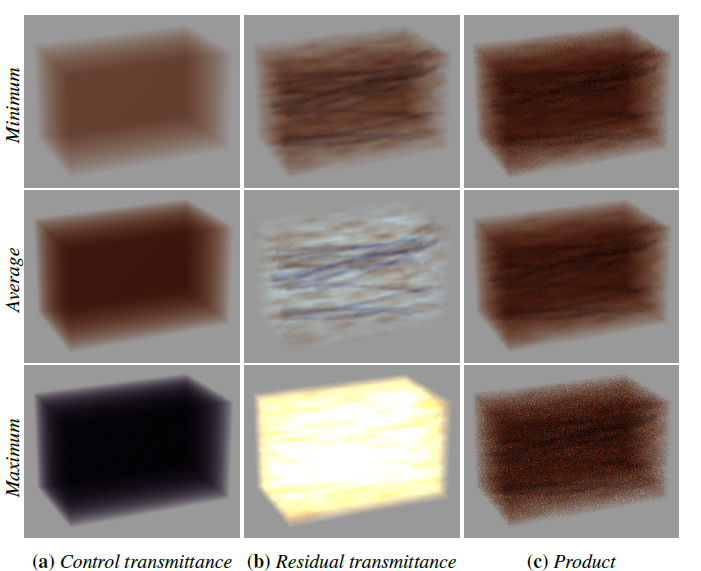
\includegraphics[width=\linewidth]{vis.PNG}
	\label{Residual ratio tracking}
	\caption{
		Residual ratio tracking in a simple procedural volume with the control transmittance (a) computed using the minimum (top), the average (middle), and the maximum (bottom) extinction coefficient in the volume. The residual transmittance (b) used to compute the product (c) was estimated using 4 trackings only to
		emphasize the noise typical for each control extinction
	}
\end{figure}
\begin{itemize}
	\item if $\mu_c = \mu_{min} = min(\mu(x));0 \leq x \leq d)$,i.e. the control extinction is underestimating, the control transmittance systematically overestimates the real transmittance
	\item if $\mu_c = \mu_{avg} = avg(\mu(x));0 \leq x \leq d)$,the control extinction
	along the ray matches the real extinction on average. The residual tracking thus corrects only for the local over- and underestimation of the control transmittance w.r.t. the real transmittance along the ray.
	\item if $\mu_c = \mu_{max} = max(\mu(x));0 \leq x \leq d)$,the control transmittance
	systematically underestimates the real transmittance and the residual tracking thus needs to produce values greater than 1 to scale the control up.
\end{itemize}
\paragraph {\textbf{Unbiasedness of Residual Ratio Tracking}}
The unbiasedness of Residual Ratio Tracking can be demonstrated if it follows the following equation:
\begin{equation}
	\begin{aligned}
		E[T] = exp(-\int_{0}^{d}\mu(x)-\mu_cdx) = \frac{T(d)}{exp(-\mu_cd)}
	\end{aligned}
\end{equation}
Now we try to prove that conclusion.As tge proof is very similar, we can directly mimic the above proof:
\begin{equation}
	\begin{aligned}
		E[T]&=exp(-\bar{\mu_r}d)\sum_{k=0}^{\infty}\frac{(\bar{\mu_r}\int_{0}^{d}\iota(x)dx)^k}{k!}\\
		&=exp(-\bar{\mu_r}d)exp(\bar{\mu_r}\int_{0}^{d}1-\frac{\mu(x)-\mu_c}{\bar{\mu_r}}dx)\\
		&=exp(-\int_{0}^{d}\bar{\mu_r})exp(\int_{0}^{d}\bar{\mu_r}-(\mu(x)-\mu_c)dx)\\
		&=exp(-\int_{0}^{d}{\mu dx}(x)-\mu_cdx)
	\end{aligned}
\end{equation}
\subsection{Adaptive and unbiased sampling using kd-tree based space partitioning}
As it's a time-consuming process to find a new scattering event in inhomogeneous participating meadia,we use an adaptive and unbiased sampling technique using kd-tree based space. partitioning. During preprocessing, it partitions the analytical space (the bounding
box of the medium) into sub-spaces (partitions,presented in kd-tree) according to the spatial variation of the mean free path in the medium. During rendering, the locations
of the scattering events are determined adaptively using the kd-tree.
\\Here is the pseudo-code of WoodcockTracking and kdTreeFreePathSampling:
\begin{algorithm}[h]
	\caption{Pseudocode of WoodcockTracking Algorithm}
	\begin{algorithmic}[1]
		\Require
		$x_0,\vec{\omega}$:The ray starting at $x_0$ in direction $\vec{\omega}$\\
		$k_M$:The majorant extinction coefficient\\
		$(d_{min},d_{max}]$:The interval of the ray to evaluate
		\Ensure
		The free path d to the next scattering event
		\State $d\gets d_{min}$-ln(1-rand())/$k_M$ 
		\While {$d\leq d_{max}\land k(x_0+d\vec{\omega})/k_M<rand()$}
		\State $d\gets d$-ln(1-rand())/$k_M$ 
		\EndWhile
		\State \Return {d}
	\end{algorithmic}
\end{algorithm}\\

\begin{algorithm}[h]
	\caption{Pseudocode of kdTreeFreePathSampling Algorithm}
	\begin{algorithmic}[1]
		\Require
		$x_0,\vec{\omega}$:The ray starting at $x_0$ in direction $\vec{\omega}$
		\Ensure
		The free path d to the next scattering event
		\While {true}
		\State $kdTreeNode\ p\gets findNextLeafNode()$ 
		\If {$p=nil$}
		\State \Return {INFINITY} \EndIf
		\State $(d_{min},d_{max})\gets intersectionBetweenRayAndNode(p)$ 
		\State $k_M\gets majorantExtinctionCoefficientStoredIn(p)$ 
		\State $d\gets WoodcockTracking(x_o,\vec{\omega},k_M,d_{min},d_{max})$ 
		\State $d_{isect}\gets INFINITY$
		 \If {$intersectionWithObjectSurfaces(x_0,\vec{\omega},p$)}
		 \State $d_{isect} \gets distanceToTheIntersection()$ \EndIf
		 \If {$d \geq d_{isect}$}
		 \State \Return {IntersectionEvent} \EndIf
		 \If {$d < d_{max}$}
		 \State \Return {d} \EndIf
		\EndWhile
	\end{algorithmic}
\end{algorithm}
\subsubsection{Unbiased Sampling and Space Partitioning}
\paragraph{\textbf{Strategy}}
Suppose the ray starting at $x_0$ in direction $\vec{\omega}$ passes through two adjacent partitions i and j, with $k_M^{(i)}$ and $k_M^{(j)}$ being their majorant extinction coefficients. Let the distances from $x_0$ to the intersections with those partitions be s, q, and t.\\
First,to sample the free path in the interval $(s,t]$,we first deal with the $(s,q])$ by using WoodcockTracking Algorithm,and if the free pathexceeds q, we rewind the free path back to q and proceed to interval $(q,t]$ and use that algorithm again.By rewinding the free path back to q, we can ensure the unbiasedness of the sampling.
\paragraph{\textbf{Proof of Unbiasedness}}
To prove unbiasedness, we need to show taht we can obtain the free path d with probability:
\begin{equation}
	\begin{aligned}
		&P(x'=x_0 + d\vec{\omega}\land s<d\leq t) = e^{-\tau(x_0+s\vec{\omega},x')}k(x')\\
		&P(d>t)= e^{-\tau(x_0+s\vec{\omega},x_0+t\vec{\omega})}
	\end{aligned}
\end{equation}
First, we obtain $d_1$ during the sampling for the first interval (s,q] with the probability:
\begin{equation}
	\begin{aligned}
		&P(x'=x_0 + d_1\vec{\omega}\land s<d_1\leq q) = e^{-\tau(x_0+s\vec{\omega},x')}k(x')\\
		&P_1(d_1>q)= e^{-\tau(x_0+s\vec{\omega},x_0+q\vec{\omega})}
	\end{aligned}
\end{equation}
Similarily, we obtain $d_2$ during the sampling for the second interval (q,t]
\begin{equation}
	\begin{aligned}
		&P(x'=x_0 + d_2\vec{\omega}\land q<d_2\leq t) = e^{-\tau(x_0+q\vec{\omega},x')}k(x')\\
		&P_1(d_2>t)= e^{-\tau(x_0+q\vec{\omega},x_0+t\vec{\omega})}
	\end{aligned}
\end{equation}
Since the sampling for the second interval is executed if and only if $d_1$ exceeds q during the sampling for the first interval, we obtain
\begin{equation}
	\begin{aligned}
		P(x'=x_0 + d\vec{\omega}\land s<d\leq q)
		&=P_1(x'=x_0 + d\vec{\omega}\land s<d\leq q)\\
		&= e^{-\tau(x_0+s\vec{\omega},x')}k(x')\\
		P(x'=x_0 + d\vec{\omega}\land q<d\leq t)
		&=P_1(d_1>q)P_2(x'=x_0 + d\vec{\omega}\land q<d\leq t)\\
	&=e^{-\tau(x_0+s\vec{\omega},x_0+q\vec{\omega})}e^{-\tau(x_0+q\vec{\omega},x')}k(x')\\
		&=e^{-\tau(x_0+s\vec{\omega},x')}k(x')\\
		P(d>t) = P_1(d>q)P_2(d>t)
		&=e^{-\tau(x_0+s\vec{\omega},x_0+q\vec{\omega})}e^{-\tau(x_0+q\vec{\omega},x_0+t\vec{\omega})}\\
		&=e^{-\tau(x_0+s\vec{\omega},x_0+t\vec{\omega})}
		\end{aligned}
\end{equation}
\subsubsection{Unbiased Sampling and Space Partitioning}
The performance of the sampling technique shown in previous section highly depends on the partitioning. If we partition a nearly homogeneous interval, an additional iteration is required to rewind the free path to q when proceeding to the adjacent interval, and this
would be a waste compared to the case with no partitioning. On the other hand, we can have more benefit, if $k_M^{(i)}$ in a partition is much smaller than kM for the entire space. These observations would give us a stopping criterion for the partitioning process, as well as a decision criterion for the partitioning location q.
\end{document}
